\documentclass{article}
\usepackage[T1]{fontenc}
\usepackage[utf8]{inputenc}
\usepackage[margin=1in]{geometry}
\usepackage{fancyhdr} 
\usepackage{listings}
\usepackage[ruled,vlined]{algorithm2e}
\usepackage{amsthm}
\usepackage{amsfonts}
\usepackage{amssymb}
\usepackage{graphicx}
\usepackage[dvipsnames]{xcolor}
\usepackage{xy}
% \usepackage{url} % Commented out because hyperref provides similar functionality
\usepackage{parskip}
\usepackage{comment}
\usepackage{setspace}
\usepackage{enumerate}
\usepackage{multirow}
\usepackage{hyperref}
\usepackage{caption}
\usepackage{subcaption}
\usepackage{booktabs}
\usepackage{wrapfig}
\usepackage{times}

\captionsetup[figure]{font={small,it}}

\usepackage[backend=biber,style=numeric,sortcites,maxbibnames=99]{biblatex}
\addbibresource{references.bib}

\newcommand{\HRule}{\rule{\linewidth}{0.5mm}}
\newcommand{\Hrule}{\rule{\linewidth}{0.3mm}}
\newcommand{\classnum}{CS-GY 6313 B}

\makeatletter% since there's an at-sign (@) in the command name
\renewcommand{\@maketitle}{%
  \parindent=0pt% don't indent paragraphs in the title block
  \centering
  {\Large \bfseries\textsc{\@title}}
  \HRule\par%
  \textit{\@author \hfill \classnum}
  \par
}
\makeatother% resets the meaning of the at-sign (@)

\title{Assignment 2: Misleading Visualization Extra Credit} 
\author{Ivan Aristy — iae225}
% \classnum

\begin{document}
  \maketitle % prints the title block
  \thispagestyle{empty}
  % \vspace{-15pt}

\section{Extra credit}
\label{sec:sec1}

\begin{figure}[ht] % Change the position of your figure https://www.overleaf.com/learn/latex/Positioning_images_and_tables
  \centering
  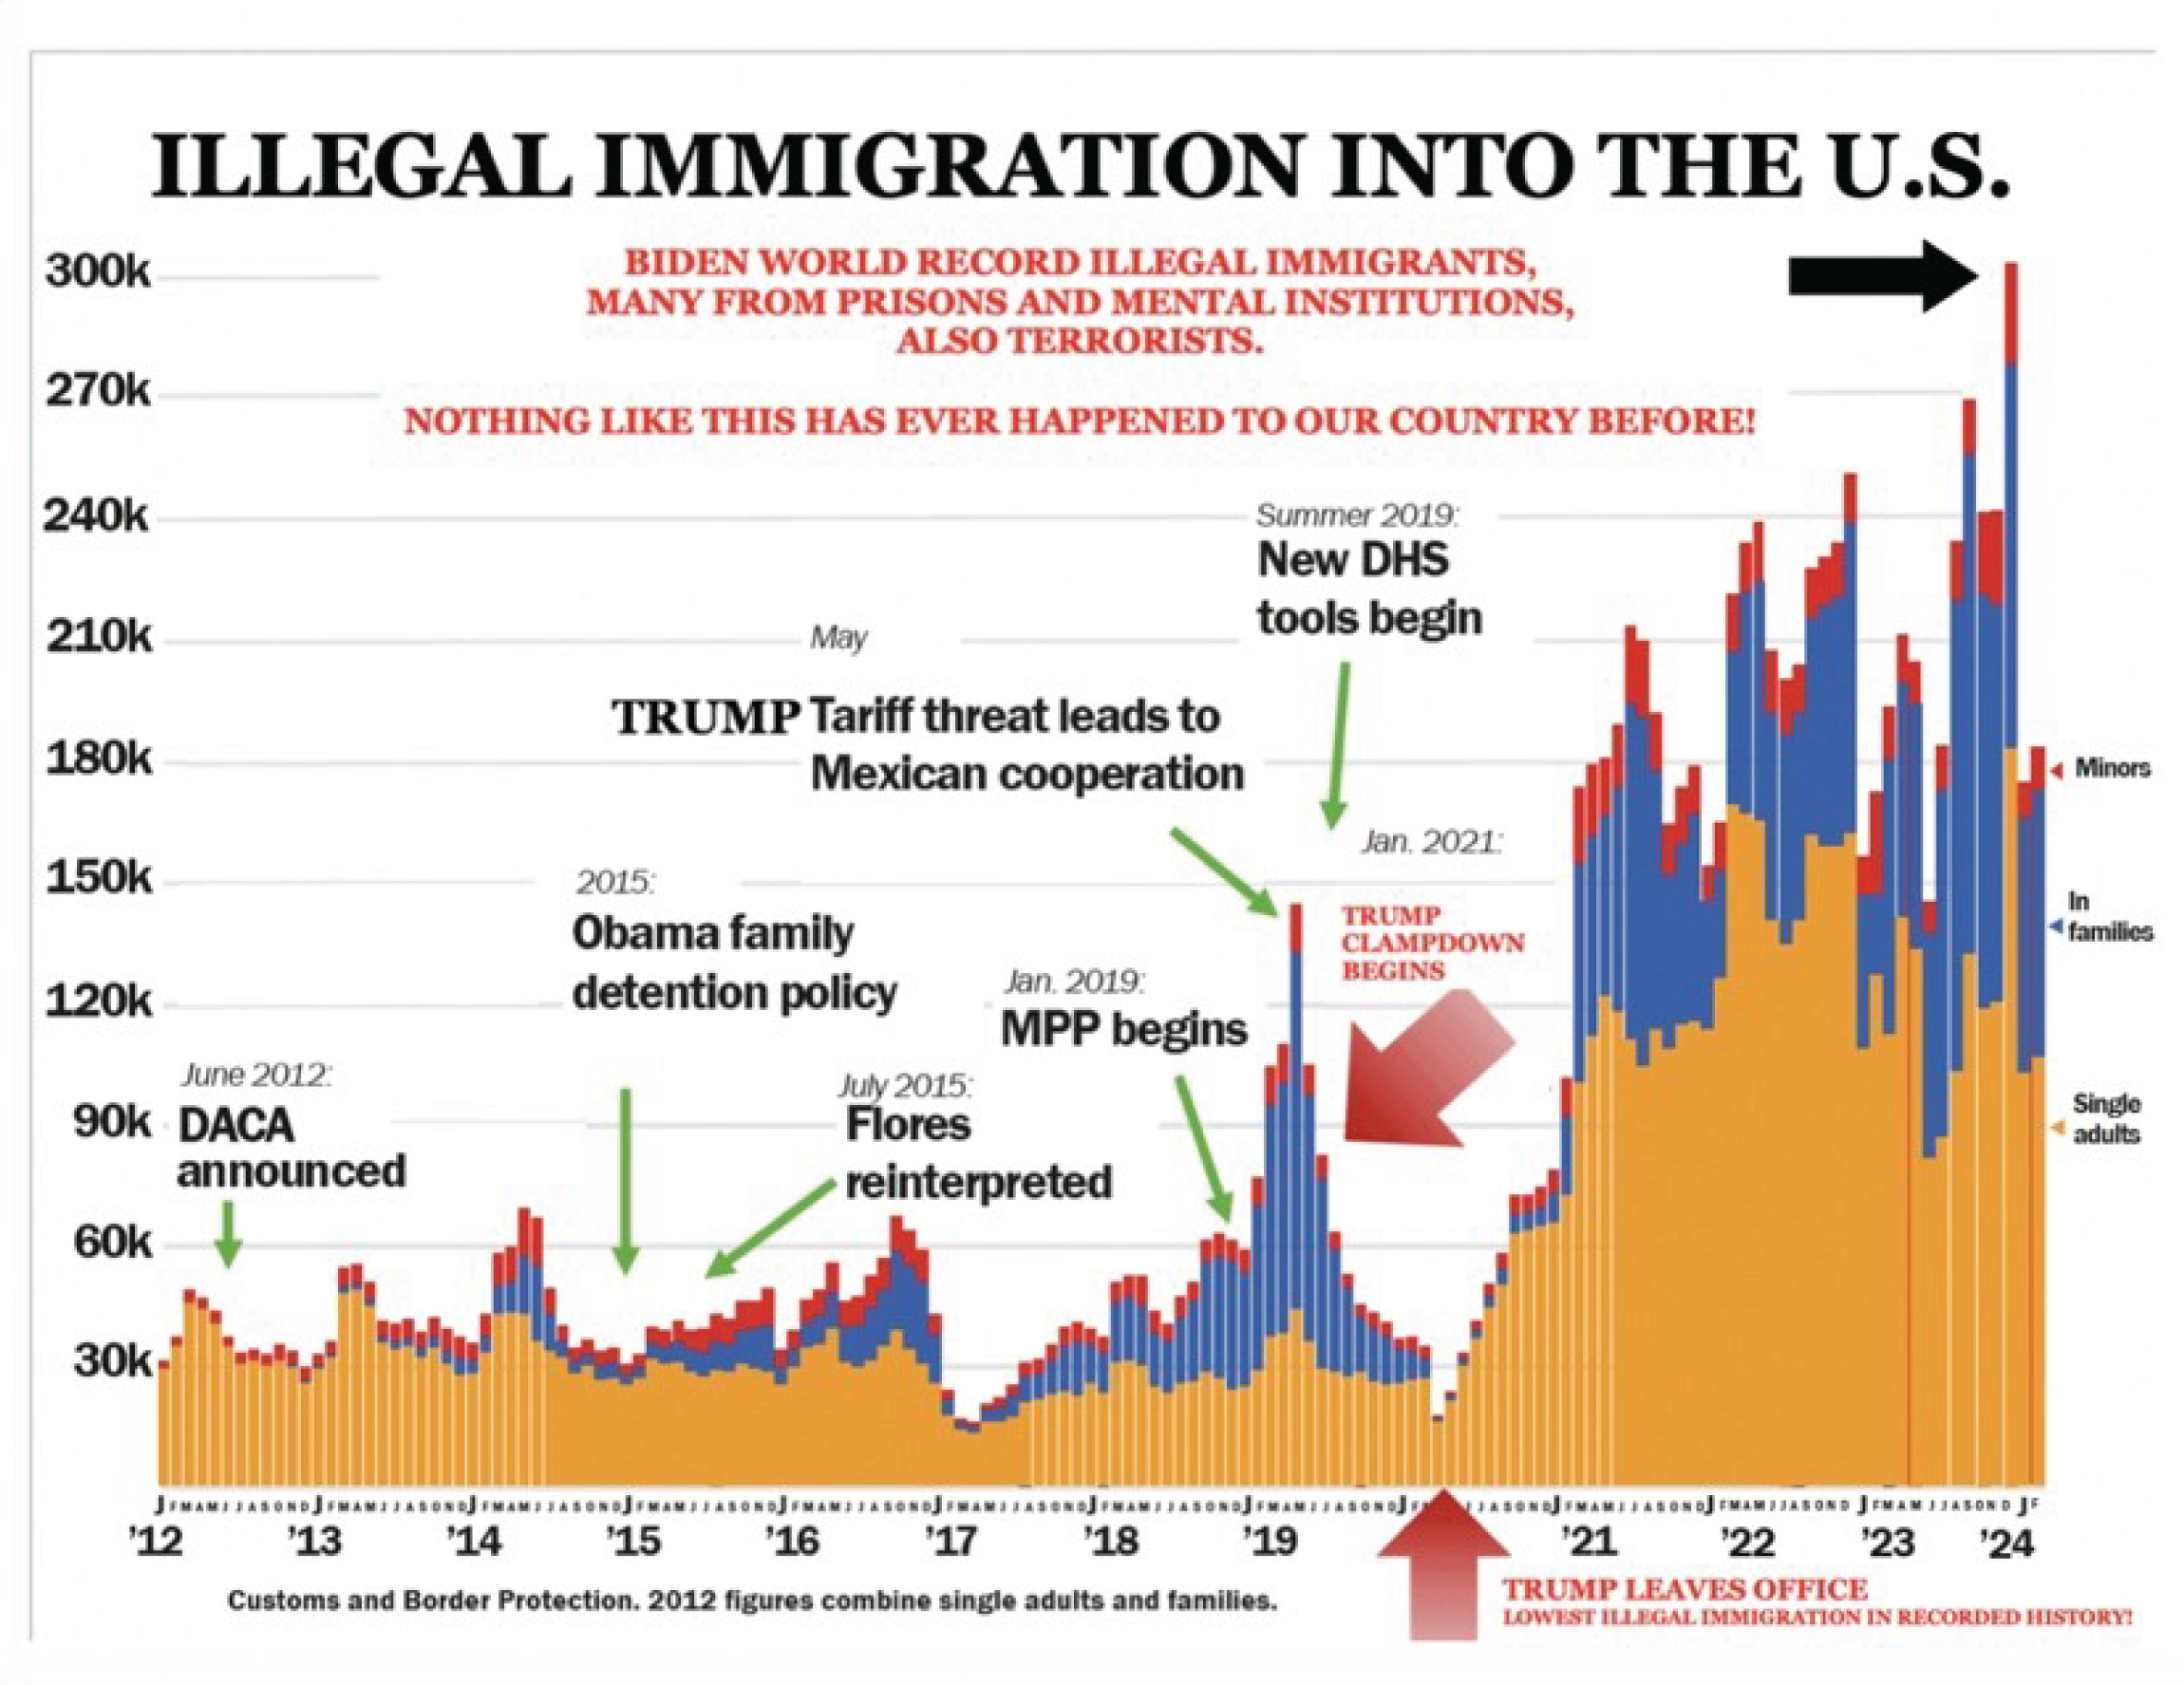
\includegraphics[width=0.75\textwidth]{figs/Trump Chart.png}
  \caption{
      Trump's Illegal Immigration Chart
  }
  \label{fig:fig1}
\end{figure}

Bar none, this is, THE WORST, THE MOST, misleading chart I have \textit{ever} seen, and probably will ever see. 
This chart is a prime example of how data can be manipulated to fit a narrative, and enrage
the american populus.

Let me list the three most egregious things about this chart:

\begin{enumerate}
  \item Trump Clapdown Begins: Wasn't there something else, BIG, going on here? Hurrican Katrina, the moon landing? 
  Can we think of anything? Surely it was just Trump's policy that caused this decline...
  OH WAIT! OH YEAH! Covid-19! The pandemic that forced billions of peoples to stay at home, and
  completely stopped all immigration... because nobody was allowed to leave their homes.
  Very convenient to leave that out. 
  \item I mean just look at the subheadng in red: "Prisions, Mental Institutions, and Terrorists"??? 
  does this graph show any of that data? Are we just assuming all of it? Where is this coming from?
  \item Also, notice how he says that Trump "left office" exactly before the big spike 
  (which was when most Covid-19 immigration control policies ended).
  However, why does he leave office in the middle of March of 2020? It is Ocotober and Biden is in office isn't he?
  He just completely disavowed the timeframe right before and after the presidential election.
  The president is still the president, during and after the new president is elected. Remember January 6th? 
  Why is this just not included as part of Trump's presidential period? He just conveniently removed an entire year's worth of 
  blame. Very on-brand.
\end{enumerate}


This can be found in trump's Twitter account, by the way. And he proudly talked about it in the Lex Friedman podcast.

But it's also here: 

\url{https://www.washingtonpost.com/politics/2024/05/23/look-trumps-misleading-inaccurate-graph-us-immigration/}

\begin{refcontext}[sorting=nyt]
\printbibliography
\end{refcontext}

\end{document}

